\documentclass[10pt,twocolumn,letterpaper]{article}
% Adjust our margins. Decrease the top margin then add double the top margin decrease as the text height addition to keep margins symmetric
\addtolength{\topmargin}{-.375in}
\addtolength{\textheight}{0.75in}

\usepackage{times}
\usepackage{epsfig}
\usepackage{graphicx}
\usepackage{amsmath}
\usepackage{amssymb}
\usepackage{float}
\usepackage{mathtools}
\usepackage[noend]{algorithmic}
% \usepackage{algorithm,caption}
\usepackage{amsmath}
\usepackage{algorithm2e}
\DeclareMathOperator*{\argmin}{arg\,min}

% Include other packages here, before hyperref.

% If you comment hyperref and then uncomment it, you should delete
% egpaper.aux before re-running latex.  (Or just hit 'q' on the first latex
% run, let it finish, and you should be clear).
\usepackage[breaklinks=true,bookmarks=false]{hyperref}


\def\cvprPaperID{****} % *** Enter the CVPR Paper ID here
\def\httilde{\mbox{\tt\raisebox{-.5ex}{\symbol{126}}}}

% Pages are numbered in submission mode, and unnumbered in camera-ready
%\ifcvprfinal\pagestyle{empty}\fi
\setcounter{page}{1}
\date{November 20, 2017}
\begin{document}

%%%%%%%%% TITLE
\title{\vspace{-0.5in}{Application Testing of Generative Adversarial Privacy}}

\author{Nicholas Johnson, Stephanie Sanchez, Vishal Subbiah\\
Stanford University\\
Computational and Mathematical Engineering\\
{nickj@stanford.edu, ssanche2@stanford.edu, svishal@stanford.edu}
% For a paper whose authors are all at the same institution,
% omit the following lines up until the university
% Additional authors and addresses can be added with ``\and'',
% just like the second author.
% To save space, use either the email address or home page, not both
}
\maketitle
%\thispagestyle{empty}

%%%%%%%%% ABSTRACT
%\begin{abstract}
  

%\end{abstract}

%%%%%%%%% BODY TEXT
%-------------------------------------------------------------------------
\section{Motivation}
%-------------------------------------------------------------------------
\subsection{Privacy}
There exist many online portals in which individuals post information whether it be text, photos, videos, etc. and some information can be released to third parties. With so much personal information distributed it is important to retain degrees of privacy while not affecting what is already chosen to be public information.   


%-------------------------------------------------------------------------
\subsection{Inference Attacks}
Machine learning (ML) methods serve many purposes today. The most revered applications of ML are normally coupled with benevolent intentions such as adverting cyber attacks, classifying materials in images for security and health purposes, etc. But ML methods do not necessarily have to be applied for favorable causes. Inference attacks, for instance, are adversary learning methods that can infer private information about public information or data. For this reason it is essential to protect privacy by deterring adversarial machine learning. 

%-------------------------------------------------------------------------
\subsection{Generative Adversarial Privacy (GAP)}
To protect the privacy of public data we have implemented a model, generative adversarial privacy (GAP), that distorts data. This enables the protection of sensitive information by obscuring generative adversarial networks (GANs) inferences of sensitive data and while not affecting the inference of nonsensitive attributes.  


%-------------------------------------------------------------------------
\section{Methods}
We have three functions and one metric as seen in figure \ref{fig:architecture}. The functions are E,G,S for encoder, gender classifier, and smile classifier respectively. A distortion metric D is included to allow for further constraints on the encoder function. We developed a multiple tiered approach of increasing complexity in order to make the problem tractable in the time alloted. We consider the encoder and classifiers as distinct entities for the sake of the GAP architecture. As such we tried two different autoencoder strategies and one classifier strategy for the milestone.

\begin{figure}[h]
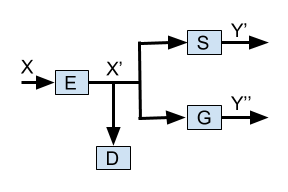
\includegraphics[width=\columnwidth]{Milestone_Graphics__2_.png}
\centering
\caption{GAP Architecture}
\label{fig:architecture}
\end{figure}
%-------------------------------------------------------------------------
\subsection{Data Preprocessing}
The images are of various sizes so we reshaped them all to 256 by 256 pixels with 3 color channels. The labels provided for smile were used as is but for some reason the gender labels had 3 categories. The third category only had a handful of samples so we removed these from our data set since we weren't able to discover the source of this unexpected anomaly. 256 by 256 was chosen based on the average sizes of the dataset. Also, it fits well in case we use a pretrained neural network, such as ResNets or VGG-Net provided by PyTorch, where we crop the images to 224 by 224.

%-------------------------------------------------------------------------
\subsection{Shallow Classifiers}
Classifying smiles and gender is a project in it's own right \cite{CNN}. However, since this course is not dedicated to deep learning we are more interested in using image classifiers as a piece of a larger whole in order to probe applications of adversarial learning. Following that methodology we implemented a two layer neural network as a place holder for deeper neural networks for the final report. This allows for initial verification of the code architecture and easier machine learning troubleshooting due to faster run times.

%-------------------------------------------------------------------------
\subsection{Compressive Encoders}
We know that neural nets can be susceptible to pixel attacks \cite{PixelAttack}. In practice we perceive this to be more information than would be available to a real world generator. However, compressive algorithms provide an interesting non-reversible information distorting encoder. In this course we evaluated two methods with which to implement this encoder. The first is PCA, where we reconstruct our image tensor via the first d principle eigenvectors for each color channel. The other method we considered is to evaluate all three channels simultaneously via a k-means compression algorithm.

%-------------------------------------------------------------------------
\subsection{Shallow Autoencoders}
By the universal approximation theorem, neural networks can reproduce any function under the appropriate constraints \cite{UA}. There is existing research in which an alternating optimization scheme is performed to calculate an explicit encoder function \cite{IA}. We are looking to set up a neural network autoencoder as an attempt to avoid this oscillating optimization scheme and create a more widely applicable product for performing GAP in practice. As such, a first step was showing that we are able to back propagate through the architecture of multiple neural networks to appropriately optimize their respective loss functions.  

%-------------------------------------------------------------------------

\section{Experimental Results}
%-------------------------------------------------------------------------
\subsection{Reproducing Previous Results as a Baseline}
Our initial goal was to reproduce the results seen in \cite{IA} based on their open source code. However, we were not able to get the test cases to agree with the documentation and in correspondance with the author learned he will be busy through the duration of the course. We still intend to compare our final results to theirs to evaluate the effectiveness of our model.

%-------------------------------------------------------------------------
\subsection{Shallow Neural Net Classifiers}
\begin{figure}[h]
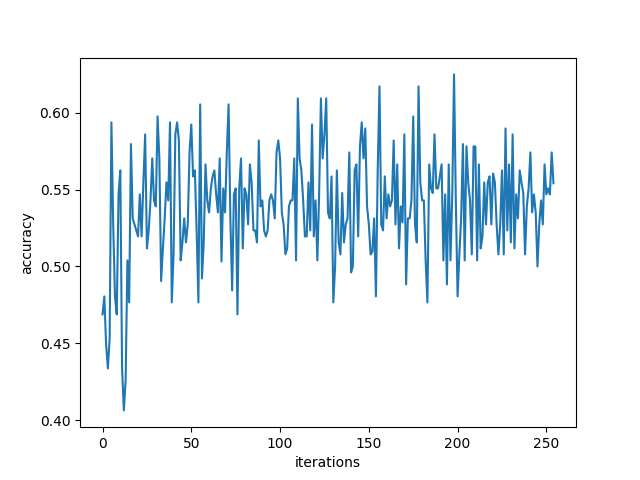
\includegraphics[width=\columnwidth]{gender_acc.png}
\centering
\caption{Gender accuracy with unmodified input data.}
\label{fig:gender_acc}
\end{figure}

\begin{figure}[h]
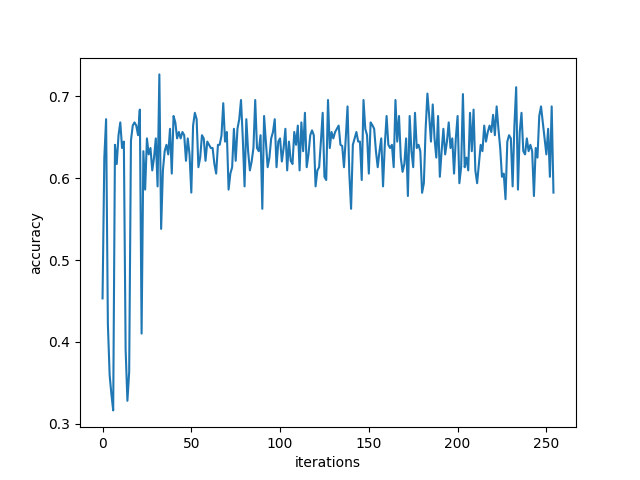
\includegraphics[width=\columnwidth]{smile_acc.png}
\centering
\caption{Smile accuracy with unmodified input data.}
\label{fig:smile_acc}
\end{figure}

For our gender and smile classifiers, G and S respectively. We were able to achieve an accuracy of approximately (55\%, 63\%), as shown in figures \ref{fig:gender_acc} and \ref{fig:smile_acc}, using our shallow 1 hidden layer neural net structure on the unmodified input data. We used this same architecture for G and S in the below experiments on the encoder function E.

%-------------------------------------------------------------------------
\subsection{PCA Encoder}
We used PCA to form a low rank approximation of each color channel of each image. For the purposes of our milestone we used 256 principle eigenvectors to prove that the framework functions appropriately with this autoencoder. This generated no effects in the results as it provided a full rank matrix. There will be experimentation with fewer eigenvectors. 

%We were able to see an accuracy of (number1,number2) at the output of our classifiers, with a total system accuracy of (number3). This is anticipated because reducing the amount of information passed to the neural networks should reduce how effective they are.

%-------------------------------------------------------------------------
\subsection{Shallow Neural Net Autoencoder}
We use our 1 hidden layer autoencoder, with the cross entropy loss function to confirm that we could train a three neural network system in the architecture outlined in \cite{GAP}. Using 15 epochs in training our classifiers for every epoch of the entire system we were able to yield an accuracy of (55\%, 63\%) at the output of our classifiers, with a total system accuracy of 37\%. We can see that the autoencoder has no effect as seen in the smile accuracy in figure \ref{fig:btr_smile}. This suggests that without more accurate classifiers it will be difficult to determine the effect of of the autoencoder.
\begin{figure}[h]
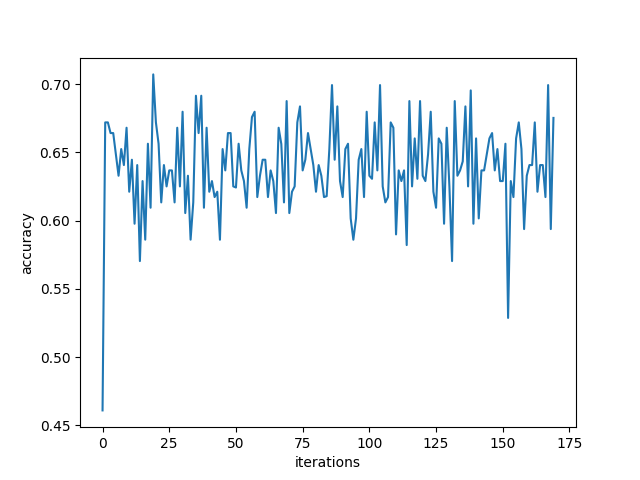
\includegraphics[width=\columnwidth]{smile_acc_all.png}
\centering
\caption{Smile accuracy with autoencoder.}
\label{fig:btr_smile}
\end{figure}
%-------------------------------------------------------------------------
\section{Next Steps}
%-------------------------------------------------------------------------
\subsection{Tune Models and Apply Deep Neural Nets}
One of the primary next steps is to improve the results of the gender and smile models by utilizing a more appropriate architecture such as a convolution neural network and optimize parameters. Additionally, 
deepening the classifiers and autoencoder could improve accuracy in addition to more accurately representing real world adversaries. Lastly, there will be experimentation with various numbers of eigenvectors with PCA to analyze any effects/changes in final results. 
%-------------------------------------------------------------------------
\subsection{Exploratory Steps}
Once we have completed the above tasks we have achieved our proof of concept for GAP application and can compare to alternative methods in the literature. Then, pending the time remaining there are a variety of directions to extend the project. There is loss function identification, to evaluate if our loss function is achieving the true privacy measure we desire. Another direction is to explore different distortion metrics which we include in our loss function as a penalty term to further constrain the encoder function. Then a sensitivity analysis on the number of epochs the classifiers have to learn from the perturbed data output from the encoder. One final option is to add random noise to make our encoder non-reversible which additionally limits the available information to the classifiers. \\
 

An interesting experiment would be to start with an externally trained deep neural network classifier and let it adapt to the perturbed input data. The accuracy could then be compared to the neural network classifiers trained during the GAP process to determine relative performance. 
%-------------------------------------------------------------------------
\section{Contributions}
Vishal has previous experience with neural networks and Pytorch so he has established the framework which we will leverage in our experiments.
Stephanie has worked on the two neural network classifiers. 
Nick reviewed background literature and contributed to setting up the GCP system for training the deep neural networks.
%-------------------------------------------------------------------------

\begin{thebibliography}{9}
\bibitem{CNN} 
Ari Ekmekji
\textit{Convolutional Neural Networks for Age and Gender Classification}. 

\bibitem{IA} 
Jihun Hamm
\textit{Minimax Filter: Learning to Preserve Privacy from Inference Attacks}. 

\bibitem{Privacy} 
Ke Xu, Tongyi Cao, Swair Shah, Crystal Maung, Haim Schweitzer
\textit{Cleaning the Null Space:A Privacy Mechanism for Predictors}. 

\bibitem{GAP}
Chong Huang, Peter Kairouz, Xiao Chen, Lalitha Sankar, and Ram Rajagopal
\textit{Context-Aware Generative Adversarial Privacy}

\bibitem{UA}
G. Cybenko
\textit{Approximation by superpositions of a sigmoidal function}

\bibitem{PixelAttack}
Jiawei Su, Danilo Vasconcellos Vargas, Sakurai Kouichi
\textit{One pixel attack for fooling deep neural networks}

\end{thebibliography}
\end{document}

